\documentclass[]{article}
\usepackage{lmodern}
\usepackage{amssymb,amsmath}
\usepackage{ifxetex,ifluatex}
\usepackage{fixltx2e} % provides \textsubscript
\ifnum 0\ifxetex 1\fi\ifluatex 1\fi=0 % if pdftex
  \usepackage[T1]{fontenc}
  \usepackage[utf8]{inputenc}
\else % if luatex or xelatex
  \ifxetex
    \usepackage{mathspec}
  \else
    \usepackage{fontspec}
  \fi
  \defaultfontfeatures{Ligatures=TeX,Scale=MatchLowercase}
\fi
% use upquote if available, for straight quotes in verbatim environments
\IfFileExists{upquote.sty}{\usepackage{upquote}}{}
% use microtype if available
\IfFileExists{microtype.sty}{%
\usepackage{microtype}
\UseMicrotypeSet[protrusion]{basicmath} % disable protrusion for tt fonts
}{}
\usepackage[margin=1in]{geometry}
\usepackage{hyperref}
\hypersetup{unicode=true,
            pdftitle={Anchoring effects on charitable donation solicitations},
            pdfauthor={Asif, Haroon, Kevin, K.C.},
            pdfborder={0 0 0},
            breaklinks=true}
\urlstyle{same}  % don't use monospace font for urls
\usepackage{graphicx,grffile}
\makeatletter
\def\maxwidth{\ifdim\Gin@nat@width>\linewidth\linewidth\else\Gin@nat@width\fi}
\def\maxheight{\ifdim\Gin@nat@height>\textheight\textheight\else\Gin@nat@height\fi}
\makeatother
% Scale images if necessary, so that they will not overflow the page
% margins by default, and it is still possible to overwrite the defaults
% using explicit options in \includegraphics[width, height, ...]{}
\setkeys{Gin}{width=\maxwidth,height=\maxheight,keepaspectratio}
\IfFileExists{parskip.sty}{%
\usepackage{parskip}
}{% else
\setlength{\parindent}{0pt}
\setlength{\parskip}{6pt plus 2pt minus 1pt}
}
\setlength{\emergencystretch}{3em}  % prevent overfull lines
\providecommand{\tightlist}{%
  \setlength{\itemsep}{0pt}\setlength{\parskip}{0pt}}
\setcounter{secnumdepth}{0}
% Redefines (sub)paragraphs to behave more like sections
\ifx\paragraph\undefined\else
\let\oldparagraph\paragraph
\renewcommand{\paragraph}[1]{\oldparagraph{#1}\mbox{}}
\fi
\ifx\subparagraph\undefined\else
\let\oldsubparagraph\subparagraph
\renewcommand{\subparagraph}[1]{\oldsubparagraph{#1}\mbox{}}
\fi

%%% Use protect on footnotes to avoid problems with footnotes in titles
\let\rmarkdownfootnote\footnote%
\def\footnote{\protect\rmarkdownfootnote}

%%% Change title format to be more compact
\usepackage{titling}

% Create subtitle command for use in maketitle
\newcommand{\subtitle}[1]{
  \posttitle{
    \begin{center}\large#1\end{center}
    }
}

\setlength{\droptitle}{-2em}
  \title{Anchoring effects on charitable donation solicitations}
  \pretitle{\vspace{\droptitle}\centering\huge}
  \posttitle{\par}
  \author{Asif, Haroon, Kevin, K.C.}
  \preauthor{\centering\large\emph}
  \postauthor{\par}
  \predate{\centering\large\emph}
  \postdate{\par}
  \date{April 13, 2017}


\begin{document}
\maketitle

\section{Abstract}\label{abstract}

Charitable fundraising efforts typically make use of suggested donation
amounts. While this practice is quite common across various techniques
and organizations there exists little research regarding optimizing
these suggested amounts. This gap in knowledge is particularly
concerning given the strong donor preference for utilizing suggested
amounts in fundraising efforts. To this end we set about conducting a
lab experiment to gather additional information regarding the
effectiveness of the anchoring technique on soliciting donations. We
sought to measure the effect of the anchor on donation participation and
donation amounts. We found little evidence for a preference on suggested
donation amounts in the lab experiments, though that could be attributed
to the small sample sizes and small donation amounts. In our experiment
because there was no significant preference over anchorage amounts we
did find some evidence that increased anchors (50\% vs 25\%) did lead to
larger fundraising amounts. In addition we also found evidence
supporting previous research that donors respond more favorably to round
suggested donations as opposed to non-round (50\% vs 37\%). In a second
study we looked to examine the same effects where we simulated increased
wealth by doubling the endowment effect of the lab setup but results
proved inconclusive.

\newpage

\section{Introduction}\label{introduction}

Charity organizations employ a wide and varied set of strategies when
seeking donations including appeals to sentimentality, appeals to logic,
peer pressure, and an ever-increasing array of creative stunts such as
the Ice Bucket Challenge for ALS research. However, the tried and true
method of direct mailing of fundraising still exists whether it be in
paper or electronic format. How can fundraisers make these efforts more
successful? Well, if we are to borrow a concept from behavioral
economics perhaps the answer is as simple as increasing the suggested
donation amount. This strategy attempts to take advantage of a cognitive
bias known as anchoring. But just how effective is this technique in
practice and is there a limit or a point of diminishing return? This
experiment seeks to measure the extent of changes in response rate and
donation amount when changes in suggested donation amount occur. We will
begin by analyzing the current research and theories in this area. After
that we will discuss the hypotheses of our experiment. We then cover the
experimental design focusing on treatment, subject selection and
randomization, important covariates, and outcome measures. Next we
discuss the results of two related studies we conducted. We conclude
with a discussion of the results and some issues noted during the
experiment. The paper includes an appendix with the regression output
for the studies.

\section{Theory}\label{theory}

The concept of anchoring was first proposed by Amos Tversky and Daniel
Kahneman.\footnote{\url{http://people.hss.caltech.edu/~camerer/Ec101/JudgementUncertainty.pdf}}
They define anchoring as a psychological heuristic or shortcut that when
individuals are making uncertain decisions of a quantitative nature they
are unduly influenced by anchors or readily available numbers. This
effect is most easily demonstrated in negotiations where studies have
shown that the opening offer has a stronger influence on the outcome of
negotiations that counteroffers.\footnote{\url{http://www.sciencedirect.com/science/article/pii/S0749597897927138}}
But the effect can extend to even random anchors. In a study conducted
by Dan Ariely he found that when he asked participants to write the last
two digits of their social security number and then have them bid on
objects such as wine and computer equipment with unknown values, those
with higher last two social security numbers submitted bids 60-120
percent higher.\footnote{\url{http://ww2.cfo.com/human-capital-careers/2004/06/avoiding-decision-traps/}}

Previous research has shown the pros and cons of anchoring approaches in
this context. In a paper by Verhaert and Van den Poel they went on to
show heterogeneous effects depending on the lifecycle of the
donor.\footnote{\url{http://wps-feb.ugent.be/Papers/wp_10_666.pdf}} In
that study they showed evidence that new donors and donors who had not
donated in an extend amount of time responded positively to anchors
associated with their most recent donation whether to that charity or
another. While active donors responded most positively to an anchor
suggesting the average donation amount. The study was interesting in its
revelation that some donors maintain an internal reference anchor that
if violated could have negative impact on donation participation.

Additional research by Reiley and Samek on the topic of suggested
donations found evidence that donors responded more positively to round
or expected intervals as opposed to non round numbers.\footnote{\url{http://spihub.org/site/resource_files/publications/spi_wp_142_samek.pdf}}
For example their study found that donors would be more likely to donate
in a scenario suggesting \$100 as opposed to \$95 despite \$100 being a
larger amount. Their study also found some evidence supporting the
theory of downward sloping demand in regards to suggested donation
amounts. That is for each suggested donation amount in increasing order
they found donors less likely to respond. This is certainly an
interesting finding because it would speak to a diminishing return on
anchoring points and may again provide further evidence of internal
anchoring points in the donor that if fundraisers are looking to raise
the most money should be cognizant of. Reiley and Samek also found that
given an ask string of donation amounts, donors strongly favored
suggested amounts despite always having the option to write in an amount
suggesting that the amount of thought that goes into a suggested
donation should be seriously considered.

\section{Hypothesis}\label{hypothesis}

\begin{enumerate}
\def\labelenumi{\arabic{enumi}.}
\tightlist
\item
  Increased Donation Amounts: recipients of fundraising solicitations
  with higher suggested donation amounts who choose to donate will
  donate larger sums.
\item
  Decreased Donation Participation: recipients of fundraising
  solicitations with higher suggested donations amounts will choose not
  to donate more often.
\item
  Decreased Donation for Abnormal Suggestions: recipients of fundraising
  solicitations with non round amounts will choose not to donate more
  often.
\end{enumerate}

Given the same fundraising message but with a larger suggested donation,
recipients influenced by the anchoring effect will choose to donate
larger sums. In cases of donation solicitation especially where the
recipients are unfamiliar with the cause or its effectiveness their
ability to generate a reasonable donation amount will be limited and
thus we expect them to be highly influenced by the suggested amount. For
the same reason, we may expect lower donation participation as
participants evaluate that anchor point as an unmanageable request even
though they could actively choose to donate less.

\section{Experimental Design}\label{experimental-design}

\subsection{Study 1}\label{study-1}

This study sought to analyze the effects of providing subjects with
average donation rate information to see how it would affect donation
rate and amounts. In addition, the study also looked at the effect of
presenting subjects with non-round or anticipated amounts and how that
affects donation rate and amount. Subjects were recruited via Mechanical
Turk and directed to fill out a survey on the Qualtrics platform for
which they would be paid 5 cents with the ability to earn an additional
60 cents by completing the survey successfully.

Subjects were requested to fill out a survey that asked 6 questions
intended to gather covariate information which will be discussed later,
perform a proofreading task, and finally were presented with the option
to donate their bonus reward to a charity. The proofreading task served
two purposes: 1. To provide an endowment effect wherein the subject
believes they have earned the bonus amount and are thus more likely to
respond as if the money was already theirs. 2. To prime the subject to
be empathetic to future donation solicitation. This was done to simulate
donation information being provided by charities in fundraising efforts
and to increase donation rates to decrease variance in response rate to
improve statistical power.

\subsubsection{Treatment}\label{treatment}

In this experiment design the primary treatment was the average donation
rate presented to subjects during the solicitation question in the
survey. The donation solicitation along with response options can be
found below. Participants who selected option 2 could enter a donation
percentage amount.

\begin{figure}[htbp]
\centering
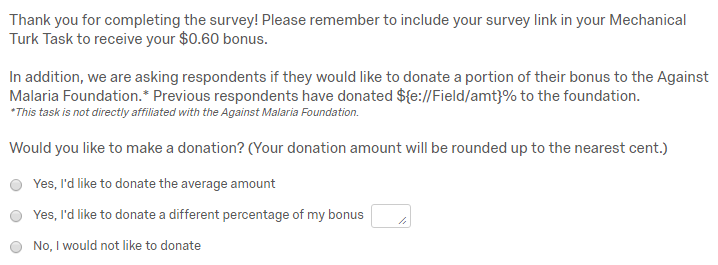
\includegraphics{treatment.PNG}
\caption{}
\end{figure}

\subsubsection{Subjects}\label{subjects}

As previously mentioned subjects were recruited from Mechanical Turk but
respondents were limited to only users from the United States. The
sample characteristics can be found below.

\subsubsection{Covariates}\label{covariates}

Covariate information was primarily gathered through the Qualtrics
survey platform. As most responses were solicited from the respondents
accuracy cannot be guaranteed and most covariates reflect self-reported
values. The following list of covariates was gathered:

\begin{itemize}
\tightlist
\item
  Age
\item
  Gender
\item
  State of Residence
\item
  Latitude/Longitude coordinates
\item
  Income level
\item
  Whether or not respondents had donated in the previous year
\item
  Employment status
\item
  Time spent on proofreading task
\item
  Number of grammatical errors identified in task
\end{itemize}

\subsubsection{Outcomes}\label{outcomes}

The potential outcome measure of primary interest was donation amount.
As a secondary measure, we would also record donor response with any
donation \textgreater{}0 equaling 1 and no donation = 0. Outcomes were
gathered based on subject responses to the Qualtrics survey.

\subsection{Study 2}\label{study-2}

Study 2 repeated the same exact experiment design but the advertised and
delivered bonus was doubled to study the potential effect of simulated
increased wealth on donation behavior as it related to our previous
outcome measures of donation amount and donation response.

\section{Results}\label{results}

Our results consist of two related studies. In the first study we
examined the impact of suggested donation amounts on donation
participation and donation amounts (measured in percent) when users were
endowed with a 60 cent bonus. Study 2 repeats the same process but with
\$1.20 bonus in attempt to see if behavior changes with larger endowment
effects or simulated wealth. As we will discuss we don't believe that
was the effect we found but instead that the users we motivated to
partake in study 2 were different.

\subsection{Study 1}\label{study-1-1}

Study 1 consisted of 196 observations of Mechanical Turk workers based
in the United States over in the month of April 2017.

Prior to performing our analysis, we did a covariate check in order to
examine the balance of a subset of covariates. The covariates examined
were:

\begin{itemize}
\tightlist
\item
  Proofreading Score
\item
  Gender
\item
  Age
\item
  Whether or not respondents had donated in the previous year
\item
  Number of grammatical errors identified in task) across all three
  groups
\end{itemize}

Our covariate test passed despite our relatively small sample size,
suggesting that the three groups are well-balanced. You can see a
summary of mean values for various covariates in table 1.

\begin{table}[!htbp] \centering 
  \caption{Summary Table of Key Covariates} 
  \label{} 
\begin{tabular}{@{\extracolsep{5pt}} cccccc} 
\\[-1.8ex]\hline 
\hline \\[-1.8ex] 
group & proofread & gender & age & prev\_donate & grammar\_score \\ 
\hline \\[-1.8ex] 
$1$ & 298.50 (27.54) & 0.46 (0.06) & 39.86 (1.55) & 0.72 (0.05) & 2.67 (0.17) \\ 
$2$ & 325.18 (32.35) & 0.35 (0.06) & 36.90 (1.57) & 0.75 (0.05) & 2.54 (0.17) \\ 
$3$ & 274.02 (24.92) & 0.31 (0.06) & 40.00 (1.75) & 0.85 (0.05) & 2.92 (0.17) \\ 
\hline \\[-1.8ex] 
\end{tabular} 
\end{table}

For our analysis, we ran four separate regressions:

\begin{itemize}
\tightlist
\item
  \(Y_i = \beta_0 + \beta_1 *proofread + \beta_2 *male + \beta_3 *age + \beta_4 *previouslydonated + \beta_5 *grammarscore + \beta_6 *group2 + \beta_7 *group3\)
\item
  \(Y_i = \beta_0 + \beta_1 *group2 + \beta_2 *group3\)
\end{itemize}

where \(Y_i\) is the donation percentage of respondents

\begin{itemize}
\tightlist
\item
  \(Y_i = \beta_0 + \beta_1 *proofread + \beta_2 *male + \beta_3 *age + \beta_4 *previouslydonated + \beta_5 *grammarscore + \beta_6 *group2 + \beta_7 *group3\)
\item
  \(Y_i = \beta_0 + \beta_1 *group2 + \beta_2 *group3\)
\end{itemize}

where \(Y_i\) is the binary variable measuring whether a respondent
donated or not

The regression output can be found in Table 6 in the appendix.

Our regressions suggest that those who donated spent more time
proofreading. One way that this could be interpreted is that those who
were more careful during the survey were more likely to be impacted by
the essay in the survey, which describes the issue of malaria. This may
have led to an stronger empathetic response amongst careful respondents
when they were asked to donate to a nonprofit that addresses the issue
of malaria.

Another interesting (and perhaps unsurprising) finding in our
regressions is that those who donated in the previous year were more
likely to donate during our study. This was the case for all three
groups involved in the study.

When examining donation rates amongst all three groups, we found that
Group 3 (50\% suggested donation) and Group 1 (25\% suggested donation)
had a somewhat similar rate of donation and Group 2 (37.5\% suggested
donation) had the lowest rate of donation of the three groups. This
result is interesting, as we would expect the rate of donation to
decrease from Group 1 to Group 2 and then from Group 2 to Group 3 if the
hypothesis of downward sloping demand was true. This result does echo
results found in Reiley and Samek's study. One likely explanation for
this result is that subjects may prefer to donate when the suggested
amount is a rounded percentage.

In regards to the donation amount (in percentages), Group 3 donated the
most on average (controlling for all other variables in the regressions)
and Group 2 donated the least. This is likely due to the high fraction
of non-donors in Group 2 as compared to the other two groups. This also
due to respondents strong preference to donate the suggested donation
amount as opposed to a write in amount. You can see the percentage of
users who donated the suggested amount in each group. (Group 2 is the
non round suggestion).

\begin{table}[!htbp] \centering 
  \caption{Study 1 Donation Activity} 
  \label{} 
\begin{tabular}{@{\extracolsep{5pt}} ccc} 
\\[-1.8ex]\hline 
\hline \\[-1.8ex] 
Group & Donors Selecting Suggested Donation & Mean Donation \% \\ 
\hline \\[-1.8ex] 
$1$ & $79.31$ & $27.76$ \\ 
$2$ & $27.27$ & $28.73$ \\ 
$3$ & $65.22$ & $49.13$ \\ 
\hline \\[-1.8ex] 
\end{tabular} 
\end{table}

\subsection{Study 2}\label{study-2-1}

Study 2 consisted of 99 observations of Mechanical Turk workers based in
the United States over the month of April 2017.

Again we begin with an analysis of covariate balance for study 2. We see
slightly less balance in study 2 primarily due to the decreased number
of participants allowing a wider variance.

\begin{table}[!htbp] \centering 
  \caption{Summary Table of Key Covariates} 
  \label{} 
\begin{tabular}{@{\extracolsep{5pt}} cccccc} 
\\[-1.8ex]\hline 
\hline \\[-1.8ex] 
group & proofread & gender & age & prev\_donate & grammar\_score \\ 
\hline \\[-1.8ex] 
$1$ & 241.46 (30.98) & 0.36 (0.08) & 37.38 (2.08) & 0.67 (0.08) & 2.67 (0.24) \\ 
$2$ & 261.62 (35.33) & 0.45 (0.09) & 35.64 (1.72) & 0.76 (0.08) & 2.91 (0.25) \\ 
$3$ & 303.08 (35.35) & 0.48 (0.10) & 34.89 (1.85) & 0.70 (0.09) & 2.48 (0.29) \\ 
\hline \\[-1.8ex] 
\end{tabular} 
\end{table}

The regression output can be found in Table 7 in the appendix.

The results from this study confound many of the results found in the
previous study. We see that the time spent proofreading has an estimated
negative impact on both likelihood to donate and amount donated though
these results are not statistically significant they are in the opposite
direction than study 1.

We see that previous donation history still has an estimated positive
impact on both likelihood to donate and amount donated although the
effect is far weaker than the one estimate in study 1.

When examining donation rates amongst all three groups, we again found
that Group 3 (50\% suggested donation) and Group 1 (25\% suggested
donation) had a somewhat similar rate of donation although now Group 2
(37.5\% suggested donation) had the highest rate of donation of the
three groups. This result is the direct opposite of findings of study 1
and confounds those results. We theorize that we may be seeing evidence
of heterogeneous treatment effects where the respondents attracted in
study 2 responded more positively to non round suggestions perhaps
giving them more authenticity than round numbers though this would need
to be investigated further.

In regards to the donation amount (in percentages), Group 2 donated the
most on average (controlling for all other variables in the regressions)
and Group 1 donated the least. This is likely due to Group 2 having the
highest response rate as well as some variance due to small sample size.
The one consistent result is the respondent preference for the suggested
donation amount. You can see the percentage of users who donated the
suggested amount in each group. (Group 2 is the non round suggestion).

\begin{table}[!htbp] \centering 
  \caption{Study 2 Donation Activity} 
  \label{} 
\begin{tabular}{@{\extracolsep{5pt}} ccc} 
\\[-1.8ex]\hline 
\hline \\[-1.8ex] 
Group & Donors Selecting Suggested Donation & Mean Donation \% \\ 
\hline \\[-1.8ex] 
$1$ & $90$ & $32.50$ \\ 
$2$ & $66.67$ & $35.50$ \\ 
$3$ & $57.14$ & $47.14$ \\ 
\hline \\[-1.8ex] 
\end{tabular} 
\end{table}

We did some further analysis on the covariates between the two studies
which can be seen in Table 5. The breakdown in self reported income
levels does seem to suggest that we recruited more lower income
individuals with the promise of a larger bonus in Study 2. We also
compared the same covariates that we examined in the randomization
checks and while there is no statistical difference between the groups
we still theorize there is some unobserved heterogeneity that makes
these groups different in substantial ways that may explain some of the
confounding results we observe in our outcomes variables. We suspect
this is a factor primarily due to the difference in the amount of time
it took for HITs to complete on Mechanical Turk. While for Study 1 our
HITs remained open for days at a time. Study 2's HIT was completed in a
matter of hours. The alternative conclusion is that the difference in
results is attributable to the difference in bonus amounts.

\includegraphics{Final_Paper_files/figure-latex/unnamed-chunk-6-1.pdf}

\begin{table}[!htbp] \centering 
  \caption{Summary Table of Key Covariates} 
  \label{} 
\begin{tabular}{@{\extracolsep{5pt}} cccccc} 
\\[-1.8ex]\hline 
\hline \\[-1.8ex] 
study & proofread & gender & age & prev\_donate & grammar\_score \\ 
\hline \\[-1.8ex] 
Study 1 & 300.39 (16.60) & 0.38 (0.03) & 38.87 (0.93) & 0.77 (0.03) & 2.70 (0.10) \\ 
Study 2 & 264.99 (19.47) & 0.42 (0.05) & 36.12 (1.11) & 0.71 (0.05) & 2.70 (0.15) \\ 
\hline \\[-1.8ex] 
\end{tabular} 
\end{table}

\section{Discussion}\label{discussion}

\subsection{Experimental Concerns}\label{experimental-concerns}

\subsubsection{Endowment effect
concerns}\label{endowment-effect-concerns}

Among the respondents in our study 1 and study 2 data there were 18
subjects who completed the proofreading task in under 60 seconds which
potentially indicates that they did not give it proper attention. The
concern here is that if users did not actually perform the proofreading
task they may not have treated the donation question the same having not
properly received the endowment effect as well as the secondary effect
of generating empathy for the charity. We have chosen not to remove the
respondents but instead have controlled for this as a covariate. As we
saw from our previous analysis there is some evidence to support the
hypothesis that increased time spend on the proofreading task did lead
to more donation activity. Below is a histogram of the number of
respondents who completed the task under 60 seconds broken into 10
second intervals.

\includegraphics{Final_Paper_files/figure-latex/unnamed-chunk-8-1.pdf}

\subsubsection{Attrition}\label{attrition}

Due to the nature of our experiment design randomization occurred just
before treatment and outcome measurement. Essentially there was no room
for attrition. We did have individuals who dropped out of the survey
prior to randomization and exposure to treatment and we discarded those
results as there were no outcomes to measure. We may be subject to some
self selection which might limit the generalizability of the results but
we have no concerns regarding differential attrition.

\subsubsection{Exclusion restriction}\label{exclusion-restriction}

Our experiment design called for creating an endowment effect and in
that process we also tried to induce empathy but as all users were
equally exposed to these we do not suspect any exclusion restrictions of
exposure to treatment. All users were exposed to the same exact
treatment question with the only change being the number.

\subsubsection{Non-interference}\label{non-interference}

There are a couple of non-interference concerns though we have little
evidence of them. The major theme is that users are discussing the study
either in person or through online messaging boards. There was some
discussion of the study on messaging boards we could find but it was
regarding a typo in our second study and seemed to occur after the
closure of the study. If there was a violation of non-interference of it
could certainly bias the results depending on the effects of the
interference but we are assuming if this did occur the effects are
negligible.

\subsection{External Validity}\label{external-validity}

As we were unable to find a partner charity organization to work with we
were forced to adapt to a more lab based experiment design. The big
concern here is how generalizable these results become under the
specific conditions they were gathered. The pool of respondents on
Mechanical Turk are certainly different in characteristics than the
general donor pool of charities whom could use this information in
fundraising efforts (though based on self reported previous donation
rates our pool compares just slightly worse than the average American
population based on IRS tax data). Another factor is that despite an
attempt to create an endowment effect, ultimately the donation decision
being made was based off of money not yet received and of a very small
amount. Effects may differ under larger donation amounts. We theorize
that this small number effect was what prevented us from finding
downward sloping demand at higher suggested donations as was found in
other studies. If our results were to hold at larger scales then
potentially the highest suggested donation amount would receive equal
donation activity to lower donation amounts. Our most confident result
was in the preference for round numbers as we feel the experiment as
designed still has valid things to say regarding this effect. Although
our results are inconclusive with the second study providing some
evidence of the opposite effect we feel given a higher powered study
this effect could be reasonably estimated.

\subsection{Future Work}\label{future-work}

This study has provided interesting insights but there is still room to
be gained. Below are a few things we would recommend as additional
follows that we ourselves would have taken on given more time and
budget:

\begin{enumerate}
\def\labelenumi{\arabic{enumi}.}
\tightlist
\item
  The first area for additional research would be to conduct a similar
  study in a field setting where we would not need to validate the
  effect of endowment effects and could gain causal inference about
  actual donor behavior.
\item
  Based on the data we have gathered so far the first step would be to
  power up the experiment by gathering more observations. While some of
  our findings are on the cusp of statistical significance others could
  benefit from a larger study.
\item
  Increasing the number of suggested donation treatments would be
  instructive to better understand the ``demand'' curve for donations.
  While we have some evidence of the predicted downward slope we cannot
  say for sure that the slope is not in fact flat.
\item
  There are also other interesting interaction effects that could be
  explored through a factorial design such as with the solicitation
  style i.e.~more specific, individual type stories to elicit a warm
  glow in donors, data-driven stories to elicit unbridled altruism, etc.
\end{enumerate}

\section{Conclusion}\label{conclusion}

We would like to revisit the hypotheses previoulsy posed as we draw some
conclusion regarding these studies.

\begin{enumerate}
\def\labelenumi{\arabic{enumi}.}
\tightlist
\item
  Increased Donation Amounts: recipients of fundraising solicitations
  with higher suggested donation amounts who choose to donate will
  donate larger sums.
\item
  Decreased Donation Participation: recipients of fundraising
  solicitations with higher suggested donations amounts will choose not
  to donate more often.
\item
  Decreased Donation for Abnormal Suggestions: recipients of fundraising
  solicitations with non round amounts will choose not to donate more
  often.
\end{enumerate}

Study 1 found some evidence for hypothesis 1 with the round donation
amounts. Both the simple and covariate controlled models in Table 6
found a signifant positive effect (at the 10\% level unadjusted for
multiple tests) for donation percentage for group 3 over the baseline of
group 1 which were the 50\% and 25\% levels respectively. The hypothesis
did not hold for group 2 when including non donators and even when
factoring them out the mean donation percentage for group was nearly
identical to group 1. Study 2 found similar effects though less
statistically significant due to a smaller number of observations. Mean
donations increased from group 1 to group 2 to group 3 and all groups
had over 50\% of donors who donated choosing the suggested amounts. This
could be evidence of the anchoring effect or the preference of users to
avoid cognitive cost in determining the amount to donate.

For hypothesis 2 we found little to no evidence of this when comparing
group 1 to group 3 where donation rates were nearly identical. There was
a difference in group 2 donation rates but this is a more related to the
3rd hypothesis which we will cover next. Study 2 did not produce any
statistically significant differences in donation rates among the three
groups. This hypothesis is well grounded in economic theory and common
sense would tell us that we could not just increase the suggested amount
infinitely and expect no change in donation percentages. There are a few
theories as to what may explain these results. First, we did not have
enough price points to establish a ``donation demand'' curve. Second,
due to the nature of endowing the individuals with and asking for a
percentage of that amount we guaranteed that all respondents could
donate at least that much whereas in a true donation solicitation with
fixed amounts some suggested donation amounts may exceed the available
discretionary income of the individual. Lastly, because of the
experiment nature users may not have experienced the same loss aversion
when donating amounts due to a lack of endowment effect and the small
nature of donation request (at most \$1.20).

We identified some evidence of hypothesis 3 in study 1. In the covariate
controlled regression the effect of the non round donation amount (37\%)
was significantly negative (at the 10\% level unadjusted for multiple
tests). This data also shows up in the number of donors who chose to
donate at that level preferring to donate a written in amount. The only
instance in both studies where the suggested donation amount was not
favored by donors. Study 2 actually found evidence directly refuting the
finding from study 1 with the non round amound producing the most
donations though this result did not achieve statistical significance.
This was a surprising finding and most certainly due to some unobserved
heterogeneity between our study 1 participants and study 2 participants
but perhaps warranting of further research to see if there certain
individuals more or less likely to respond non round amounts. There are
two competing theories with non round amounts. One, that individuals
donors all things equal prefer to minimize cognitive costs when choosing
to donate and non round amounts produce an anchor that is more difficult
to compare with their internal assessment of how much they are willing
to donate. The second theory is that individuals in viewing a suggested
donation amount attribute more authenticity to a non round amount as
they assess the likelihood of a round amount naturally occurring to be
small. This theory would affect users with weak internal anchors more so
than those with a strong donation reference point.

We believe that further research into this area is required as the
existing literature still leaves many questions to answer. We also
believe the concerns of generalizability could be laid to rest with a
fully funded, high powered field experiment in this area and we hope to
see continued research on this topic.

\newpage

\section{References}\label{references}

Kristensen, Henrik, and Tommy Gärling. ``The Effects of Anchor Points
and Reference Points on Negotiation Process and Outcome.''
Organizational Behavior and Human Decision Processes 71, no. 1 (1997):
85-94. Accessed April 2, 2017. \url{doi:10.1006/obhd.1997.2713}.

Reiley, David, and Anya Savikhin Samek. ``How Do Suggested Donations
Affect Charitable Gifts? Evidence from a Field Experiment in Public
Broadcasting.'' SSRN Electronic Journal. Accessed April 2, 2017.
\url{doi:10.2139/ssrn.2702174}.

Teach, Edward. ``Avoiding Decision Traps.'' CFO. May 11, 2015. Accessed
April 02, 2017.
\url{http://ww2.cfo.com/human-capital-careers/2004/06/avoiding-decision-traps/}.

Tversky, Amos, and Daniel Kahneman. ``Judgment under uncertainty:
Heuristics and biases.'' Judgment under uncertainty, September 27, 1974,
1124-131. \url{doi:10.1017/cbo9780511809477.002}.

Verhaert, Griet Alice, and Dirk Van Den Poel. ``Improving Campaign
Success Rate by Tailoring Donation Requests along the Donor Lifecycle.''
Journal of Interactive Marketing 25, no. 1 (2011): 51-63.
\url{doi:10.1016/j.intmar.2010.09.001}.

\newpage

\section{Appendix}\label{appendix}

\begin{table}[!htbp] \centering 
  \caption{Study 1 Regression} 
  \label{} 
\begin{tabular}{@{\extracolsep{5pt}}lcccc} 
\\[-1.8ex]\hline 
\hline \\[-1.8ex] 
 & \multicolumn{4}{c}{\textit{Dependent variable:}} \\ 
\cline{2-5} 
\\[-1.8ex] & \multicolumn{2}{c}{donate\_perc} & \multicolumn{2}{c}{donate\_yn} \\ 
\\[-1.8ex] & (1) & (2) & (3) & (4)\\ 
\hline \\[-1.8ex] 
 proofread &  & 0.01$^{*}$ &  & 0.0004$^{***}$ \\ 
  &  & (0.01) &  & (0.0002) \\ 
  & & & & \\ 
 genderMale &  & $-$2.47 &  & $-$0.06 \\ 
  &  & (3.42) &  & (0.07) \\ 
  & & & & \\ 
 age &  & $-$0.16 &  & $-$0.01$^{**}$ \\ 
  &  & (0.13) &  & (0.003) \\ 
  & & & & \\ 
 prev\_donateYes &  & 8.35$^{**}$ &  & 0.30$^{***}$ \\ 
  &  & (4.03) &  & (0.09) \\ 
  & & & & \\ 
 grammar\_score &  & $-$0.84 &  & $-$0.02 \\ 
  &  & (1.26) &  & (0.03) \\ 
  & & & & \\ 
 factor(group)2 & $-$2.37 & $-$3.50 & $-$0.10 & $-$0.14$^{*}$ \\ 
  & (3.69) & (3.84) & (0.08) & (0.08) \\ 
  & & & & \\ 
 factor(group)3 & 7.49$^{*}$ & 7.02$^{*}$ & $-$0.03 & $-$0.03 \\ 
  & (3.83) & (4.03) & (0.09) & (0.09) \\ 
  & & & & \\ 
 Constant & 11.67$^{***}$ & 7.12 & 0.42$^{***}$ & 0.10 \\ 
  & (2.60) & (8.05) & (0.06) & (0.17) \\ 
  & & & & \\ 
\hline \\[-1.8ex] 
Observations & 196 & 195 & 196 & 195 \\ 
R$^{2}$ & 0.04 & 0.12 & 0.01 & 0.20 \\ 
Adjusted R$^{2}$ & 0.03 & 0.03 & $-$0.003 & 0.11 \\ 
Residual Std. Error & 21.59 (df = 193) & 21.53 (df = 176) & 0.49 (df = 193) & 0.46 (df = 176) \\ 
F Statistic & 3.53$^{**}$ (df = 2; 193) & 1.37 (df = 18; 176) & 0.70 (df = 2; 193) & 2.40$^{***}$ (df = 18; 176) \\ 
\hline 
\hline \\[-1.8ex] 
\textit{Note:}  & \multicolumn{4}{r}{$^{*}$p$<$0.1; $^{**}$p$<$0.05; $^{***}$p$<$0.01} \\ 
\end{tabular} 
\end{table}

\begin{table}[!htbp] \centering 
  \caption{Study 2 Regression} 
  \label{} 
\begin{tabular}{@{\extracolsep{5pt}}lcccc} 
\\[-1.8ex]\hline 
\hline \\[-1.8ex] 
 & \multicolumn{4}{c}{\textit{Dependent variable:}} \\ 
\cline{2-5} 
\\[-1.8ex] & \multicolumn{2}{c}{donate\_perc} & \multicolumn{2}{c}{donate\_yn} \\ 
\\[-1.8ex] & (1) & (2) & (3) & (4)\\ 
\hline \\[-1.8ex] 
 proofread &  & $-$0.004 &  & $-$0.0002 \\ 
  &  & (0.01) &  & (0.0003) \\ 
  & & & & \\ 
 genderMale &  & $-$4.14 &  & $-$0.11 \\ 
  &  & (4.82) &  & (0.10) \\ 
  & & & & \\ 
 genderPrefer not to answer &  & $-$4.37 &  & $-$0.14 \\ 
  &  & (22.72) &  & (0.49) \\ 
  & & & & \\ 
 age &  & 0.15 &  & 0.01 \\ 
  &  & (0.23) &  & (0.005) \\ 
  & & & & \\ 
 prev\_donateYes &  & 2.43 &  & 0.02 \\ 
  &  & (5.22) &  & (0.11) \\ 
  & & & & \\ 
 grammar\_score &  & 1.28 &  & 0.05 \\ 
  &  & (1.83) &  & (0.04) \\ 
  & & & & \\ 
 factor(group)2 & 4.58 & 4.57 & 0.11 & 0.14 \\ 
  & (4.85) & (5.13) & (0.11) & (0.11) \\ 
  & & & & \\ 
 factor(group)3 & 3.89 & 3.65 & 0.003 & 0.03 \\ 
  & (5.13) & (5.52) & (0.12) & (0.12) \\ 
  & & & & \\ 
 Constant & 8.33$^{**}$ & $-$4.30 & 0.26$^{***}$ & $-$0.19 \\ 
  & (3.28) & (11.22) & (0.07) & (0.24) \\ 
  & & & & \\ 
\hline \\[-1.8ex] 
Observations & 99 & 99 & 99 & 99 \\ 
R$^{2}$ & 0.01 & 0.18 & 0.01 & 0.24 \\ 
Adjusted R$^{2}$ & $-$0.01 & $-$0.02 & $-$0.01 & 0.05 \\ 
Residual Std. Error & 20.50 (df = 96) & 20.57 (df = 79) & 0.46 (df = 96) & 0.44 (df = 79) \\ 
F Statistic & 0.52 (df = 2; 96) & 0.92 (df = 19; 79) & 0.59 (df = 2; 96) & 1.30 (df = 19; 79) \\ 
\hline 
\hline \\[-1.8ex] 
\textit{Note:}  & \multicolumn{4}{r}{$^{*}$p$<$0.1; $^{**}$p$<$0.05; $^{***}$p$<$0.01} \\ 
\end{tabular} 
\end{table}

\begin{table}[!htbp] \centering 
  \caption{Logistic Regressions For Donation Rates} 
  \label{} 
\begin{tabular}{@{\extracolsep{5pt}}lcccc} 
\\[-1.8ex]\hline 
\hline \\[-1.8ex] 
 & \multicolumn{4}{c}{\textit{Dependent variable:}} \\ 
\cline{2-5} 
\\[-1.8ex] & \multicolumn{4}{c}{donate\_yn} \\ 
\\[-1.8ex] & (1) & (2) & (3) & (4)\\ 
\hline \\[-1.8ex] 
 proofread &  & 0.002$^{***}$ &  & $-$0.001 \\ 
  &  & (0.001) &  & (0.002) \\ 
  & & & & \\ 
 genderMale &  & $-$0.30 &  & $-$0.71 \\ 
  &  & (0.36) &  & (0.61) \\ 
  & & & & \\ 
 genderPrefer not to answer &  &  &  & $-$14.58 \\ 
  &  &  &  & (2,399.55) \\ 
  & & & & \\ 
 age &  & $-$0.03$^{**}$ &  & 0.04 \\ 
  &  & (0.02) &  & (0.03) \\ 
  & & & & \\ 
 prev\_donateYes &  & 1.68$^{***}$ &  & 0.06 \\ 
  &  & (0.50) &  & (0.65) \\ 
  & & & & \\ 
 grammar\_score &  & $-$0.12 &  & 0.33 \\ 
  &  & (0.14) &  & (0.25) \\ 
  & & & & \\ 
 factor(group)2 & $-$0.42 & $-$0.76$^{*}$ & 0.51 & 0.91 \\ 
  & (0.36) & (0.42) & (0.52) & (0.65) \\ 
  & & & & \\ 
 factor(group)3 & $-$0.13 & $-$0.09 & 0.01 & 0.28 \\ 
  & (0.36) & (0.42) & (0.57) & (0.69) \\ 
  & & & & \\ 
 Constant & $-$0.32 & $-$2.25$^{**}$ & $-$1.06$^{***}$ & $-$4.22$^{***}$ \\ 
  & (0.24) & (1.00) & (0.37) & (1.59) \\ 
  & & & & \\ 
\hline \\[-1.8ex] 
Observations & 196 & 195 & 99 & 99 \\ 
Log Likelihood & $-$129.20 & $-$107.74 & $-$59.28 & $-$46.56 \\ 
Akaike Inf. Crit. & 264.41 & 253.49 & 124.57 & 133.11 \\ 
\hline 
\hline \\[-1.8ex] 
\textit{Note:}  & \multicolumn{4}{r}{$^{*}$p$<$0.1; $^{**}$p$<$0.05; $^{***}$p$<$0.01} \\ 
\end{tabular} 
\end{table}


\end{document}
